\documentclass{standalone}
\usepackage{tikz}
% default colors
% used in standalone pictures and when no university is selected
\definecolor{black}{HTML}{000000}
\definecolor{green}{HTML}{33BB33}
\definecolor{red}{HTML}{BB3333}
\definecolor{orange}{HTML}{BB6600}
\definecolor{blue}{HTML}{3333BB}
\definecolor{uulmaccent}{HTML}{999999}

\definecolor{uulmlogoblue}{named}{blue}
\definecolor{uulmblue}{named}{blue}

\ifdarkmode
	\colorlet{green}{green!85!white}
	\colorlet{red}{red!85!white}
	\colorlet{orange}{orange!85!white}
	\colorlet{blue}{blue!85!white}
	\setbeamercolor{section in toc shaded}{fg=black}
	\setbeamertemplate{section in toc shaded}[default][50]
\fi

% TYPICAL COMMANDS FOR LECTURES

\renewcommand{\emph}[1]{{\color{blue}\textbf{#1}}}

\newcommand{\deutsch}[1]{{\color{blue}(#1)}}
\newcommand{\deutschertitel}[1]{{\tiny\deutsch{#1}}}

\newcommand{\mycite}[1]{``#1''}
\newcommand{\mytitlesource}[1]{{\tiny\normalfont\mbox{[#1]}}}
\newcommand{\mysource}[1]{\ifthenelse{\equal{#1}{}}{}{\phantom{.}~\hfill~\mytitlesource{#1}}}

\newcommand{\todo}[1]{{\color{red}\textbf{[#1]}}}
\newcommand{\fodo}[1]{\todo{\footnote{\todo{#1}}}}
\newcommand{\todots}{\todo{\ldots}}

\newcommand{\textheightwithtitle}{.85\textheight}
\newcommand{\textheightwithouttitle}{.975\textheight}

% COMMANDS FOR PROPOSITIONAL FORMULAS AND MATHEMATICAL NOTATIONS

\newcommand{\sem}[1]{\ensuremath{\llbracket #1 \rrbracket}} % semantics brackets
\newcommand{\pand}{\wedge} % conjunction
\newcommand{\por}{\vee} % disjunction
\newcommand{\pnot}{\neg} % negation
\newcommand{\pequals}{\leftrightarrow} % biconditional
\newcommand{\npequals}{\nleftrightarrow} % exclusive disjunction
\newcommand{\mequals}{\Leftrightarrow} % equivalence (meta-level)
\newcommand{\pimplies}{\rightarrow} % conditional
\newcommand{\mimplies}{\Rightarrow} % implication (meta-level)
\newcommand{\defeq}{\vcentcolon=} % defining equals
\newcommand{\power}[1]{\mathcal{P}(#1)} % power set
\newcommand{\refslide}[1]{\hyperlink{#1}{(see Slide \autoref{#1})}} % link to slide

\usepackage{mathtools} % required for absolute value in modeling lecture
\DeclarePairedDelimiter\abs{\lvert}{\rvert} % absolute value

% COMMANDS TO INCLUDE XKCDs

\newcommand{\xkcd}[1]{
	\begin{frame}
		\centering%
		\href{https://xkcd.com/#1/}{\includegraphics[height=80mm]{#1}}
	\end{frame}
}
\newcommand{\widexkcd}[1]{
	\begin{frame}
		\centering%
		\href{https://xkcd.com/#1/}{\includegraphics[width=\linewidth]{xkcd/#1}}
	\end{frame}
}


\begin{document}
	\sffamily
	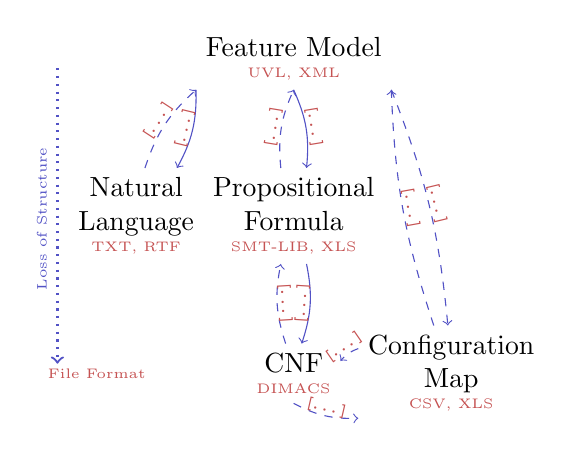
\begin{tikzpicture}
		\tikzstyle{every edge}=[font=\tiny,draw,color=blue]

		\node (topleft) at (-1,0) {};
		\node (bottomleft) at (-1,-4) {};
		\node (bottomleft2) at (-0.5,-4) {\tiny\color{red}File Format};
		
		\node (fd) at (2,0) [align=center] {Feature Model\\[-1ex]{\tiny\color{red}UVL, XML}};
		\node (nat) at (0,-2) [align=center] {Natural\\Language\\[-1ex]{\tiny\color{red}TXT, RTF}};
		\node (phi) at (2,-2) [align=center] {Propositional\\Formula\\[-1ex]{\tiny\color{red}SMT-LIB, XLS}};
		\node (cfg) at (4,-4) [align=center] {Configuration\\Map\\[-1ex]{\tiny\color{red}CSV, XLS}};
		\node (cnf) at (2,-4) [align=center] {CNF\\[-1ex]{\tiny\color{red}DIMACS}};

		\path [dotted, thick, ->] (topleft) edge node[left, rotate=90, yshift=2mm, xshift=10mm] {Loss of Structure} (bottomleft);
	
		\path [->] (fd.south west) edge[bend left=15] node[sloped,yshift=1mm] {\todots} (nat);
		\path [dashed, ->] (nat) edge[bend left=15] node[sloped,yshift=1mm] {\todots} (fd.south west); % \bakarnaturallanguage
		
		\path [->] (fd.south) edge[bend left=15] node[sloped,yshift=1mm] {\todots} (phi);
		\path [dashed, ->] (phi) edge[bend left=15] node[sloped,yshift=1mm] {\todots} (fd.south); % \czarneckithereandbackagain, \shereverseengineering

		\path [dashed, ->] (fd.south east) edge[bend left=8] node[sloped,yshift=1mm] {\todots} (cfg);
		\path [dashed, ->] (cfg) edge[bend left=8] node[sloped,yshift=1mm] {\todots} (fd.south east);

		\path [->] (phi) edge[bend left=15] node[sloped,yshift=1mm] {\todots} (cnf);
		\path [dashed, ->] (cnf) edge[bend left=15] node[sloped,yshift=1mm] {\todots} (phi);
	
		\path [dashed, ->] (cfg) edge[bend right=15] node[sloped,yshift=1mm] {\todots} (cnf);
		\path [dashed, ->] (cnf.south) edge[bend right=15] node[sloped,yshift=1mm] {\todots} (cfg);
	\end{tikzpicture}
\end{document}